\documentclass[12pt]{article}
\usepackage{tikz}
\usepackage{amsmath}
% Underlining package
\usepackage{ulem}
\usetikzlibrary{calc}
\usetikzlibrary{angles,quotes}
\usepackage[a4paper, portrait, margin=1cm]{geometry}
\usepackage{fancyhdr}

\newcommand{\HeadingAnswers}{%
\section*{\Large Name: \underline{\hspace{8cm}} \hfill Date: \underline{\hspace{3cm}}}%
\vspace{-3mm}\par
\textbf{Area of a Circle: Answers}\vspace{1pt}\hrule
}

% raise footer with page number; no header
\fancypagestyle{myfancypagestyle}{
  \fancyhf{}% clear all header and footer fields
  \renewcommand{\headrulewidth}{0pt} % no rule under header
  \fancyfoot[C] {\thepage} \setlength{\footskip}{14.5pt} % raise page number allowed min 14.5pt
}
\pagestyle{myfancypagestyle}  % apply myfancypagestyle

\newcounter{minipagecount}

\begin{document}
\HeadingAnswers
\vspace{8mm}

\begin{minipage}{0.50\textwidth}
  \refstepcounter{minipagecount}
  \noindent{(\theminipagecount)}\quad
  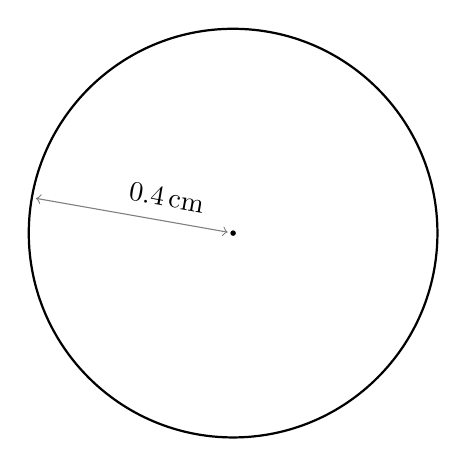
\begin{tikzpicture}[scale=1.0, baseline=(current bounding box.north)]
    \begin{scope}[rotate=0]
        \coordinate (A) at (0,0);
        % Define B using polar coordinates from A
        \coordinate (B) at ($(A) + (170:2.595)$);
        \fill (A) circle(1pt);
        \draw[thick] (A) circle (2.595);
        \draw[<->, gray, shorten <=2pt, shorten >=1.5pt]
          (A) -- (B)
          node[pos=0.35, sloped, above, fill=white, inner sep=2pt, xshift=0pt, yshift=3pt, transform shape]
          {\textcolor{black}{$0.4\,\text{cm}$}};
    \end{scope}
  \end{tikzpicture}
\end{minipage}%
\hfill
\begin{minipage}{0.45\textwidth}
  \begin{align*}
  \text{Circumference} &= 2\pi r \\
  \text{Circumference} &= 2 \times \pi \times 0.4\,\text{cm} \\
  \text{Circumference} &\approx 2.513 \,\text{cm}
  \end{align*}
\end{minipage}
\par\vspace{1cm}\begin{minipage}{0.50\textwidth}
  \refstepcounter{minipagecount}
  \noindent{(\theminipagecount)}\quad
  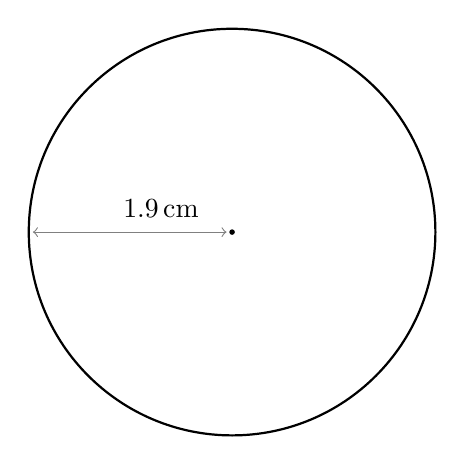
\begin{tikzpicture}[scale=1.0, baseline=(current bounding box.north)]
    \begin{scope}[rotate=0]
        \coordinate (A) at (0,0);
        % Define B using polar coordinates from A
        \coordinate (B) at ($(A) + (180:2.582)$);
        \fill (A) circle(1pt);
        \draw[thick] (A) circle (2.582);
        \draw[<->, gray, shorten <=2pt, shorten >=1.5pt]
          (A) -- (B)
          node[pos=0.35, sloped, above, fill=white, inner sep=2pt, xshift=0pt, yshift=3pt, transform shape]
          {\textcolor{black}{$1.9\,\text{cm}$}};
    \end{scope}
  \end{tikzpicture}
\end{minipage}%
\hfill
\begin{minipage}{0.45\textwidth}
  \begin{align*}
  \text{Circumference} &= 2\pi r \\
  \text{Circumference} &= 2 \times \pi \times 1.9\,\text{cm} \\
  \text{Circumference} &\approx 11.938 \,\text{cm}
  \end{align*}
\end{minipage}
\par\vspace{1cm}\begin{minipage}{0.50\textwidth}
  \refstepcounter{minipagecount}
  \noindent{(\theminipagecount)}\quad
  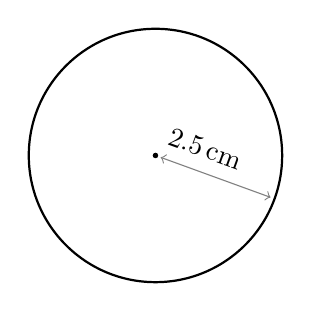
\begin{tikzpicture}[scale=1.0, baseline=(current bounding box.north)]
    \begin{scope}[rotate=0]
        \coordinate (A) at (0,0);
        % Define B using polar coordinates from A
        \coordinate (B) at ($(A) + (-20:1.609)$);
        \fill (A) circle(1pt);
        \draw[thick] (A) circle (1.609);
        \draw[<->, gray, shorten <=2pt, shorten >=1.5pt]
          (A) -- (B)
          node[pos=0.35, sloped, above, fill=white, inner sep=2pt, xshift=0pt, yshift=3pt, transform shape]
          {\textcolor{black}{$2.5\,\text{cm}$}};
    \end{scope}
  \end{tikzpicture}
\end{minipage}%
\hfill
\begin{minipage}{0.45\textwidth}
  \begin{align*}
  \text{Circumference} &= 2\pi r \\
  \text{Circumference} &= 2 \times \pi \times 2.5\,\text{cm} \\
  \text{Circumference} &\approx 15.708 \,\text{cm}
  \end{align*}
\end{minipage}
\par\vspace{1cm}\begin{minipage}{0.50\textwidth}
  \refstepcounter{minipagecount}
  \noindent{(\theminipagecount)}\quad
  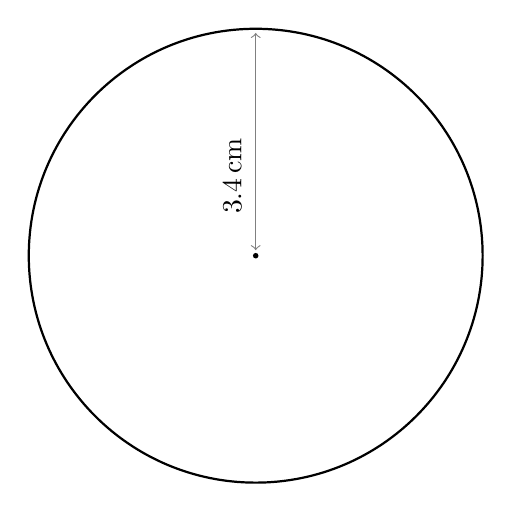
\begin{tikzpicture}[scale=1.0, baseline=(current bounding box.north)]
    \begin{scope}[rotate=0]
        \coordinate (A) at (0,0);
        % Define B using polar coordinates from A
        \coordinate (B) at ($(A) + (90:2.882)$);
        \fill (A) circle(1pt);
        \draw[thick] (A) circle (2.882);
        \draw[<->, gray, shorten <=2pt, shorten >=1.5pt]
          (A) -- (B)
          node[pos=0.35, sloped, above, fill=white, inner sep=2pt, xshift=0pt, yshift=3pt, transform shape]
          {\textcolor{black}{$3.4\,\text{cm}$}};
    \end{scope}
  \end{tikzpicture}
\end{minipage}%
\hfill
\begin{minipage}{0.45\textwidth}
  \begin{align*}
  \text{Circumference} &= 2\pi r \\
  \text{Circumference} &= 2 \times \pi \times 3.4\,\text{cm} \\
  \text{Circumference} &\approx 21.363 \,\text{cm}
  \end{align*}
\end{minipage}
\par\vspace{1cm}\begin{minipage}{0.50\textwidth}
  \refstepcounter{minipagecount}
  \noindent{(\theminipagecount)}\quad
  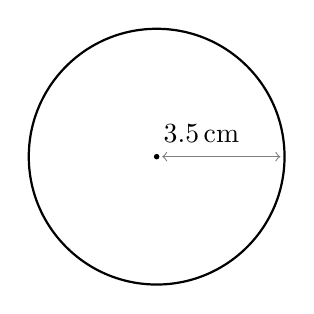
\begin{tikzpicture}[scale=1.0, baseline=(current bounding box.north)]
    \begin{scope}[rotate=0]
        \coordinate (A) at (0,0);
        % Define B using polar coordinates from A
        \coordinate (B) at ($(A) + (0:1.624)$);
        \fill (A) circle(1pt);
        \draw[thick] (A) circle (1.624);
        \draw[<->, gray, shorten <=2pt, shorten >=1.5pt]
          (A) -- (B)
          node[pos=0.35, sloped, above, fill=white, inner sep=2pt, xshift=0pt, yshift=3pt, transform shape]
          {\textcolor{black}{$3.5\,\text{cm}$}};
    \end{scope}
  \end{tikzpicture}
\end{minipage}%
\hfill
\begin{minipage}{0.45\textwidth}
  \begin{align*}
  \text{Circumference} &= 2\pi r \\
  \text{Circumference} &= 2 \times \pi \times 3.5\,\text{cm} \\
  \text{Circumference} &\approx 21.991 \,\text{cm}
  \end{align*}
\end{minipage}
\par\vspace{1cm}\begin{minipage}{0.50\textwidth}
  \refstepcounter{minipagecount}
  \noindent{(\theminipagecount)}\quad
  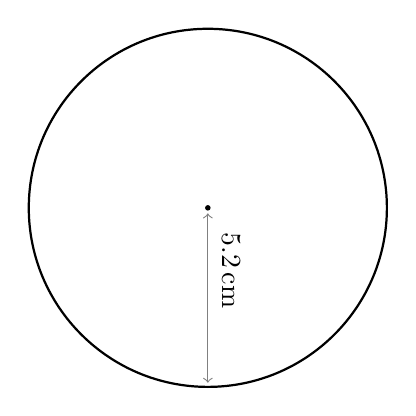
\begin{tikzpicture}[scale=1.0, baseline=(current bounding box.north)]
    \begin{scope}[rotate=0]
        \coordinate (A) at (0,0);
        % Define B using polar coordinates from A
        \coordinate (B) at ($(A) + (270:2.274)$);
        \fill (A) circle(1pt);
        \draw[thick] (A) circle (2.274);
        \draw[<->, gray, shorten <=2pt, shorten >=1.5pt]
          (A) -- (B)
          node[pos=0.35, sloped, above, fill=white, inner sep=2pt, xshift=0pt, yshift=3pt, transform shape]
          {\textcolor{black}{$5.2\,\text{cm}$}};
    \end{scope}
  \end{tikzpicture}
\end{minipage}%
\hfill
\begin{minipage}{0.45\textwidth}
  \begin{align*}
  \text{Circumference} &= 2\pi r \\
  \text{Circumference} &= 2 \times \pi \times 5.2\,\text{cm} \\
  \text{Circumference} &\approx 32.673 \,\text{cm}
  \end{align*}
\end{minipage}
\par\vspace{1cm}\begin{minipage}{0.50\textwidth}
  \refstepcounter{minipagecount}
  \noindent{(\theminipagecount)}\quad
  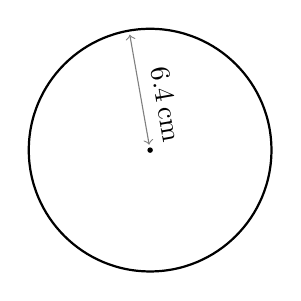
\begin{tikzpicture}[scale=1.0, baseline=(current bounding box.north)]
    \begin{scope}[rotate=0]
        \coordinate (A) at (0,0);
        % Define B using polar coordinates from A
        \coordinate (B) at ($(A) + (100:1.541)$);
        \fill (A) circle(1pt);
        \draw[thick] (A) circle (1.541);
        \draw[<->, gray, shorten <=2pt, shorten >=1.5pt]
          (A) -- (B)
          node[pos=0.35, sloped, above, fill=white, inner sep=2pt, xshift=0pt, yshift=3pt, transform shape]
          {\textcolor{black}{$6.4\,\text{cm}$}};
    \end{scope}
  \end{tikzpicture}
\end{minipage}%
\hfill
\begin{minipage}{0.45\textwidth}
  \begin{align*}
  \text{Circumference} &= 2\pi r \\
  \text{Circumference} &= 2 \times \pi \times 6.4\,\text{cm} \\
  \text{Circumference} &\approx 40.212 \,\text{cm}
  \end{align*}
\end{minipage}
\par\vspace{1cm}\begin{minipage}{0.50\textwidth}
  \refstepcounter{minipagecount}
  \noindent{(\theminipagecount)}\quad
  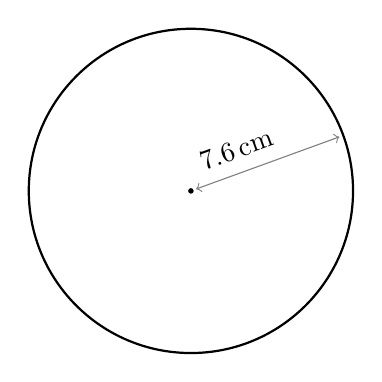
\begin{tikzpicture}[scale=1.0, baseline=(current bounding box.north)]
    \begin{scope}[rotate=0]
        \coordinate (A) at (0,0);
        % Define B using polar coordinates from A
        \coordinate (B) at ($(A) + (20:2.059)$);
        \fill (A) circle(1pt);
        \draw[thick] (A) circle (2.059);
        \draw[<->, gray, shorten <=2pt, shorten >=1.5pt]
          (A) -- (B)
          node[pos=0.35, sloped, above, fill=white, inner sep=2pt, xshift=0pt, yshift=3pt, transform shape]
          {\textcolor{black}{$7.6\,\text{cm}$}};
    \end{scope}
  \end{tikzpicture}
\end{minipage}%
\hfill
\begin{minipage}{0.45\textwidth}
  \begin{align*}
  \text{Circumference} &= 2\pi r \\
  \text{Circumference} &= 2 \times \pi \times 7.6\,\text{cm} \\
  \text{Circumference} &\approx 47.752 \,\text{cm}
  \end{align*}
\end{minipage}
\par\vspace{1cm}\begin{minipage}{0.50\textwidth}
  \refstepcounter{minipagecount}
  \noindent{(\theminipagecount)}\quad
  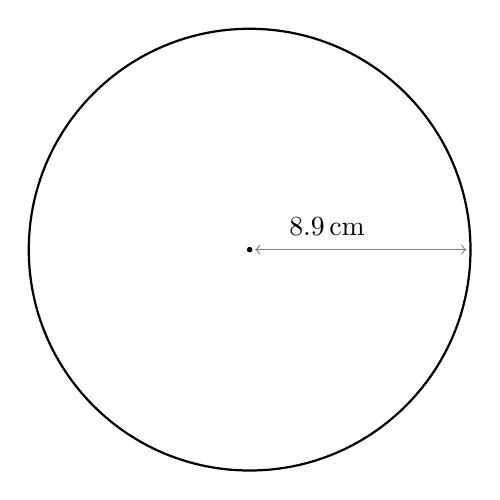
\begin{tikzpicture}[scale=1.0, baseline=(current bounding box.north)]
    \begin{scope}[rotate=0]
        \coordinate (A) at (0,0);
        % Define B using polar coordinates from A
        \coordinate (B) at ($(A) + (0:2.805)$);
        \fill (A) circle(1pt);
        \draw[thick] (A) circle (2.805);
        \draw[<->, gray, shorten <=2pt, shorten >=1.5pt]
          (A) -- (B)
          node[pos=0.35, sloped, above, fill=white, inner sep=2pt, xshift=0pt, yshift=3pt, transform shape]
          {\textcolor{black}{$8.9\,\text{cm}$}};
    \end{scope}
  \end{tikzpicture}
\end{minipage}%
\hfill
\begin{minipage}{0.45\textwidth}
  \begin{align*}
  \text{Circumference} &= 2\pi r \\
  \text{Circumference} &= 2 \times \pi \times 8.9\,\text{cm} \\
  \text{Circumference} &\approx 55.92 \,\text{cm}
  \end{align*}
\end{minipage}
\par\vspace{1cm}\begin{minipage}{0.50\textwidth}
  \refstepcounter{minipagecount}
  \noindent{(\theminipagecount)}\quad
  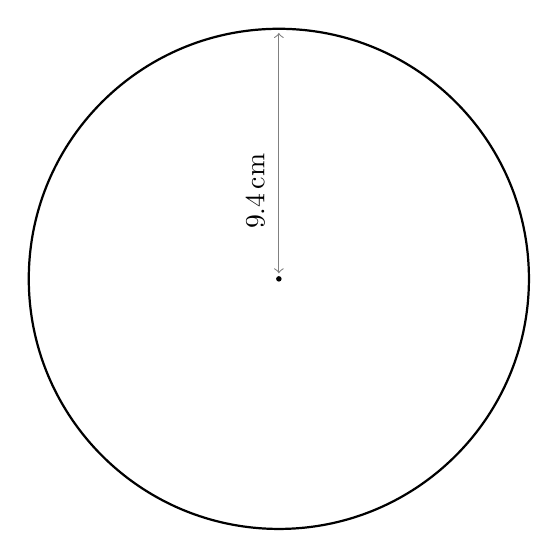
\begin{tikzpicture}[scale=1.0, baseline=(current bounding box.north)]
    \begin{scope}[rotate=0]
        \coordinate (A) at (0,0);
        % Define B using polar coordinates from A
        \coordinate (B) at ($(A) + (90:3.176)$);
        \fill (A) circle(1pt);
        \draw[thick] (A) circle (3.176);
        \draw[<->, gray, shorten <=2pt, shorten >=1.5pt]
          (A) -- (B)
          node[pos=0.35, sloped, above, fill=white, inner sep=2pt, xshift=0pt, yshift=3pt, transform shape]
          {\textcolor{black}{$9.4\,\text{cm}$}};
    \end{scope}
  \end{tikzpicture}
\end{minipage}%
\hfill
\begin{minipage}{0.45\textwidth}
  \begin{align*}
  \text{Circumference} &= 2\pi r \\
  \text{Circumference} &= 2 \times \pi \times 9.4\,\text{cm} \\
  \text{Circumference} &\approx 59.062 \,\text{cm}
  \end{align*}
\end{minipage}
\par\vspace{1cm}\begin{minipage}{0.50\textwidth}
  \refstepcounter{minipagecount}
  \noindent{(\theminipagecount)}\quad
  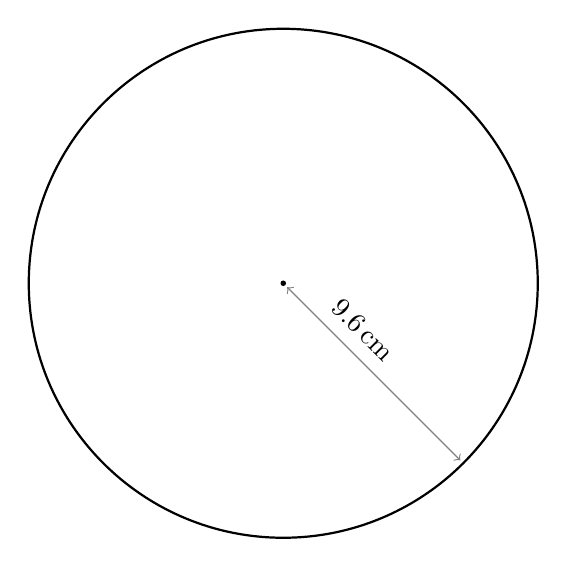
\begin{tikzpicture}[scale=1.0, baseline=(current bounding box.north)]
    \begin{scope}[rotate=0]
        \coordinate (A) at (0,0);
        % Define B using polar coordinates from A
        \coordinate (B) at ($(A) + (315:3.232)$);
        \fill (A) circle(1pt);
        \draw[thick] (A) circle (3.232);
        \draw[<->, gray, shorten <=2pt, shorten >=1.5pt]
          (A) -- (B)
          node[pos=0.35, sloped, above, fill=white, inner sep=2pt, xshift=0pt, yshift=3pt, transform shape]
          {\textcolor{black}{$9.6\,\text{cm}$}};
    \end{scope}
  \end{tikzpicture}
\end{minipage}%
\hfill
\begin{minipage}{0.45\textwidth}
  \begin{align*}
  \text{Circumference} &= 2\pi r \\
  \text{Circumference} &= 2 \times \pi \times 9.6\,\text{cm} \\
  \text{Circumference} &\approx 60.319 \,\text{cm}
  \end{align*}
\end{minipage}
\par\vspace{1cm}\begin{minipage}{0.50\textwidth}
  \refstepcounter{minipagecount}
  \noindent{(\theminipagecount)}\quad
  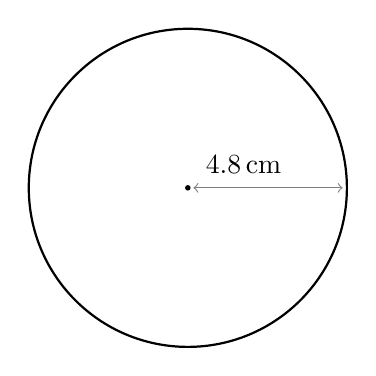
\begin{tikzpicture}[scale=1.0, baseline=(current bounding box.north)]
    \begin{scope}[rotate=0]
        \coordinate (A) at (0,0);
        % Define B using polar coordinates from A
        \coordinate (B) at ($(A) + (0:2.02)$);
        \fill (A) circle(1pt);
        \draw[thick] (A) circle (2.02);
        \draw[<->, gray, shorten <=2pt, shorten >=1.5pt]
          (A) -- (B)
          node[pos=0.35, sloped, above, fill=white, inner sep=2pt, xshift=0pt, yshift=3pt, transform shape]
          {\textcolor{black}{$4.8\,\text{cm}$}};
    \end{scope}
  \end{tikzpicture}
\end{minipage}%
\hfill
\begin{minipage}{0.45\textwidth}
  \begin{align*}
  \text{Circumference} &= 2\pi r \\
  \text{Circumference} &= 2 \times \pi \times 4.8\,\text{cm} \\
  \text{Circumference} &\approx 30.159 \,\text{cm}
  \end{align*}
\end{minipage}
\par\vspace{1cm}\begin{minipage}{0.50\textwidth}
  \refstepcounter{minipagecount}
  \noindent{(\theminipagecount)}\quad
  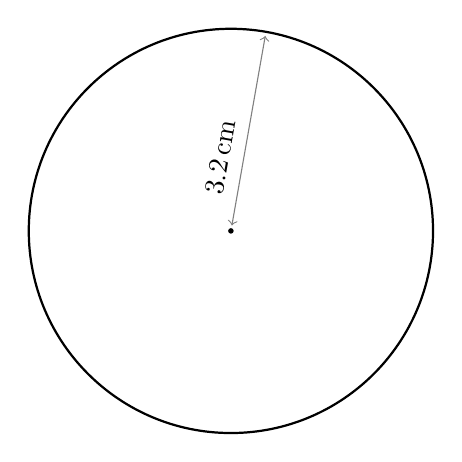
\begin{tikzpicture}[scale=1.0, baseline=(current bounding box.north)]
    \begin{scope}[rotate=0]
        \coordinate (A) at (0,0);
        % Define B using polar coordinates from A
        \coordinate (B) at ($(A) + (80:2.567)$);
        \fill (A) circle(1pt);
        \draw[thick] (A) circle (2.567);
        \draw[<->, gray, shorten <=2pt, shorten >=1.5pt]
          (A) -- (B)
          node[pos=0.35, sloped, above, fill=white, inner sep=2pt, xshift=0pt, yshift=3pt, transform shape]
          {\textcolor{black}{$3.2\,\text{cm}$}};
    \end{scope}
  \end{tikzpicture}
\end{minipage}%
\hfill
\begin{minipage}{0.45\textwidth}
  \begin{align*}
  \text{Circumference} &= 2\pi r \\
  \text{Circumference} &= 2 \times \pi \times 3.2\,\text{cm} \\
  \text{Circumference} &\approx 20.106 \,\text{cm}
  \end{align*}
\end{minipage}
\par\vspace{1cm}\begin{minipage}{0.50\textwidth}
  \refstepcounter{minipagecount}
  \noindent{(\theminipagecount)}\quad
  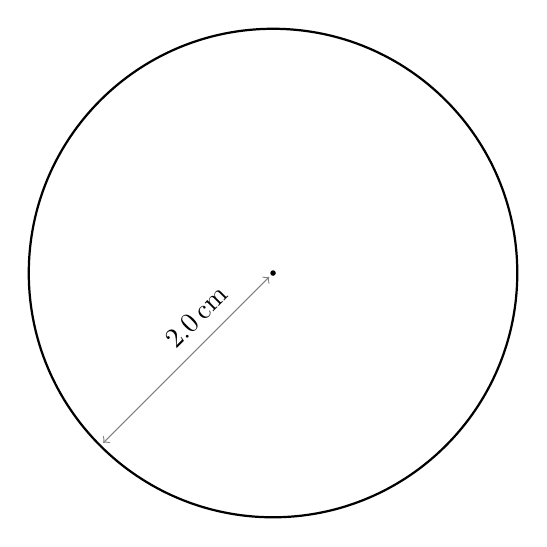
\begin{tikzpicture}[scale=1.0, baseline=(current bounding box.north)]
    \begin{scope}[rotate=0]
        \coordinate (A) at (0,0);
        % Define B using polar coordinates from A
        \coordinate (B) at ($(A) + (225:3.102)$);
        \fill (A) circle(1pt);
        \draw[thick] (A) circle (3.102);
        \draw[<->, gray, shorten <=2pt, shorten >=1.5pt]
          (A) -- (B)
          node[pos=0.35, sloped, above, fill=white, inner sep=2pt, xshift=0pt, yshift=3pt, transform shape]
          {\textcolor{black}{$2.0\,\text{cm}$}};
    \end{scope}
  \end{tikzpicture}
\end{minipage}%
\hfill
\begin{minipage}{0.45\textwidth}
  \begin{align*}
  \text{Circumference} &= 2\pi r \\
  \text{Circumference} &= 2 \times \pi \times 2.0\,\text{cm} \\
  \text{Circumference} &\approx 12.566 \,\text{cm}
  \end{align*}
\end{minipage}
\par\vspace{1cm}\begin{minipage}{0.50\textwidth}
  \refstepcounter{minipagecount}
  \noindent{(\theminipagecount)}\quad
  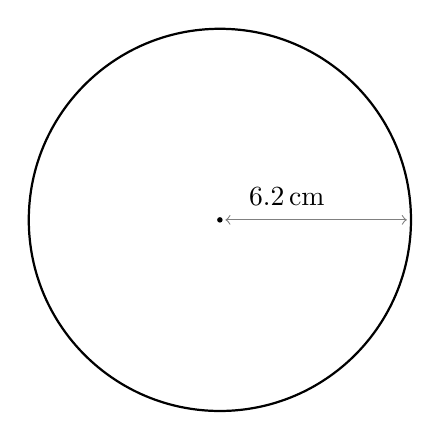
\begin{tikzpicture}[scale=1.0, baseline=(current bounding box.north)]
    \begin{scope}[rotate=0]
        \coordinate (A) at (0,0);
        % Define B using polar coordinates from A
        \coordinate (B) at ($(A) + (0:2.427)$);
        \fill (A) circle(1pt);
        \draw[thick] (A) circle (2.427);
        \draw[<->, gray, shorten <=2pt, shorten >=1.5pt]
          (A) -- (B)
          node[pos=0.35, sloped, above, fill=white, inner sep=2pt, xshift=0pt, yshift=3pt, transform shape]
          {\textcolor{black}{$6.2\,\text{cm}$}};
    \end{scope}
  \end{tikzpicture}
\end{minipage}%
\hfill
\begin{minipage}{0.45\textwidth}
  \begin{align*}
  \text{Circumference} &= 2\pi r \\
  \text{Circumference} &= 2 \times \pi \times 6.2\,\text{cm} \\
  \text{Circumference} &\approx 38.956 \,\text{cm}
  \end{align*}
\end{minipage}
\par\vspace{1cm}\begin{minipage}{0.50\textwidth}
  \refstepcounter{minipagecount}
  \noindent{(\theminipagecount)}\quad
  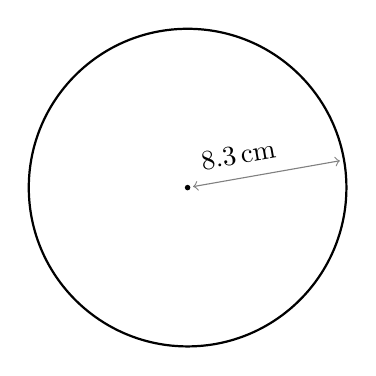
\begin{tikzpicture}[scale=1.0, baseline=(current bounding box.north)]
    \begin{scope}[rotate=0]
        \coordinate (A) at (0,0);
        % Define B using polar coordinates from A
        \coordinate (B) at ($(A) + (10:2.017)$);
        \fill (A) circle(1pt);
        \draw[thick] (A) circle (2.017);
        \draw[<->, gray, shorten <=2pt, shorten >=1.5pt]
          (A) -- (B)
          node[pos=0.35, sloped, above, fill=white, inner sep=2pt, xshift=0pt, yshift=3pt, transform shape]
          {\textcolor{black}{$8.3\,\text{cm}$}};
    \end{scope}
  \end{tikzpicture}
\end{minipage}%
\hfill
\begin{minipage}{0.45\textwidth}
  \begin{align*}
  \text{Circumference} &= 2\pi r \\
  \text{Circumference} &= 2 \times \pi \times 8.3\,\text{cm} \\
  \text{Circumference} &\approx 52.15 \,\text{cm}
  \end{align*}
\end{minipage}
\par\vspace{1cm}\begin{minipage}{0.50\textwidth}
  \refstepcounter{minipagecount}
  \noindent{(\theminipagecount)}\quad
  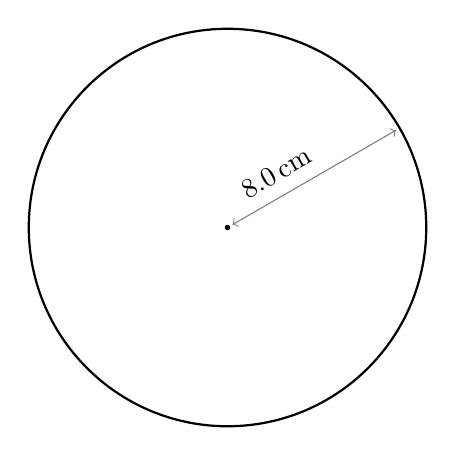
\begin{tikzpicture}[scale=1.0, baseline=(current bounding box.north)]
    \begin{scope}[rotate=0]
        \coordinate (A) at (0,0);
        % Define B using polar coordinates from A
        \coordinate (B) at ($(A) + (30:2.524)$);
        \fill (A) circle(1pt);
        \draw[thick] (A) circle (2.524);
        \draw[<->, gray, shorten <=2pt, shorten >=1.5pt]
          (A) -- (B)
          node[pos=0.35, sloped, above, fill=white, inner sep=2pt, xshift=0pt, yshift=3pt, transform shape]
          {\textcolor{black}{$8.0\,\text{cm}$}};
    \end{scope}
  \end{tikzpicture}
\end{minipage}%
\hfill
\begin{minipage}{0.45\textwidth}
  \begin{align*}
  \text{Circumference} &= 2\pi r \\
  \text{Circumference} &= 2 \times \pi \times 8.0\,\text{cm} \\
  \text{Circumference} &\approx 50.265 \,\text{cm}
  \end{align*}
\end{minipage}
\par\vspace{1cm}\begin{minipage}{0.50\textwidth}
  \refstepcounter{minipagecount}
  \noindent{(\theminipagecount)}\quad
  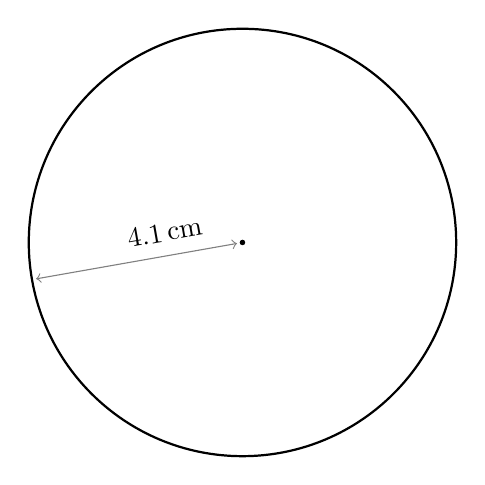
\begin{tikzpicture}[scale=1.0, baseline=(current bounding box.north)]
    \begin{scope}[rotate=0]
        \coordinate (A) at (0,0);
        % Define B using polar coordinates from A
        \coordinate (B) at ($(A) + (190:2.714)$);
        \fill (A) circle(1pt);
        \draw[thick] (A) circle (2.714);
        \draw[<->, gray, shorten <=2pt, shorten >=1.5pt]
          (A) -- (B)
          node[pos=0.35, sloped, above, fill=white, inner sep=2pt, xshift=0pt, yshift=3pt, transform shape]
          {\textcolor{black}{$4.1\,\text{cm}$}};
    \end{scope}
  \end{tikzpicture}
\end{minipage}%
\hfill
\begin{minipage}{0.45\textwidth}
  \begin{align*}
  \text{Circumference} &= 2\pi r \\
  \text{Circumference} &= 2 \times \pi \times 4.1\,\text{cm} \\
  \text{Circumference} &\approx 25.761 \,\text{cm}
  \end{align*}
\end{minipage}
\par\vspace{1cm}\begin{minipage}{0.50\textwidth}
  \refstepcounter{minipagecount}
  \noindent{(\theminipagecount)}\quad
  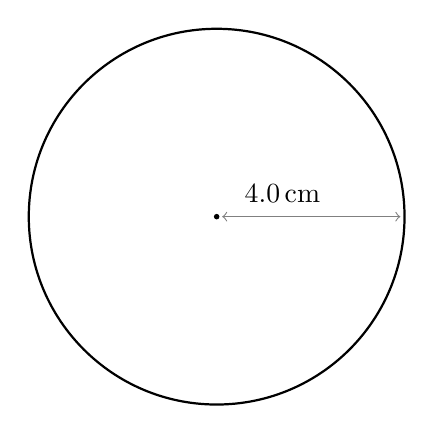
\begin{tikzpicture}[scale=1.0, baseline=(current bounding box.north)]
    \begin{scope}[rotate=0]
        \coordinate (A) at (0,0);
        % Define B using polar coordinates from A
        \coordinate (B) at ($(A) + (0:2.386)$);
        \fill (A) circle(1pt);
        \draw[thick] (A) circle (2.386);
        \draw[<->, gray, shorten <=2pt, shorten >=1.5pt]
          (A) -- (B)
          node[pos=0.35, sloped, above, fill=white, inner sep=2pt, xshift=0pt, yshift=3pt, transform shape]
          {\textcolor{black}{$4.0\,\text{cm}$}};
    \end{scope}
  \end{tikzpicture}
\end{minipage}%
\hfill
\begin{minipage}{0.45\textwidth}
  \begin{align*}
  \text{Circumference} &= 2\pi r \\
  \text{Circumference} &= 2 \times \pi \times 4.0\,\text{cm} \\
  \text{Circumference} &\approx 25.133 \,\text{cm}
  \end{align*}
\end{minipage}
\par\vspace{1cm}\begin{minipage}{0.50\textwidth}
  \refstepcounter{minipagecount}
  \noindent{(\theminipagecount)}\quad
  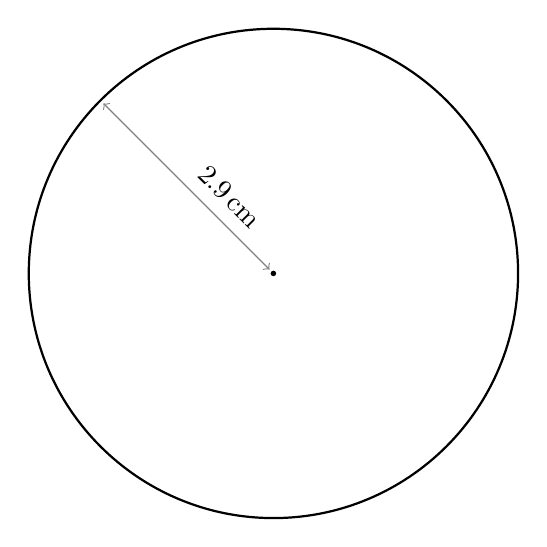
\begin{tikzpicture}[scale=1.0, baseline=(current bounding box.north)]
    \begin{scope}[rotate=0]
        \coordinate (A) at (0,0);
        % Define B using polar coordinates from A
        \coordinate (B) at ($(A) + (135:3.107)$);
        \fill (A) circle(1pt);
        \draw[thick] (A) circle (3.107);
        \draw[<->, gray, shorten <=2pt, shorten >=1.5pt]
          (A) -- (B)
          node[pos=0.35, sloped, above, fill=white, inner sep=2pt, xshift=0pt, yshift=3pt, transform shape]
          {\textcolor{black}{$2.9\,\text{cm}$}};
    \end{scope}
  \end{tikzpicture}
\end{minipage}%
\hfill
\begin{minipage}{0.45\textwidth}
  \begin{align*}
  \text{Circumference} &= 2\pi r \\
  \text{Circumference} &= 2 \times \pi \times 2.9\,\text{cm} \\
  \text{Circumference} &\approx 18.221 \,\text{cm}
  \end{align*}
\end{minipage}
\par\vspace{1cm}

\end{document}
